\chapter{Degree Anonymization over Uncertain Graphs}
\label{chp:d}
In this chapter, I will briefly review the degree anonymization tehcniques I developed for uncertain graphs. These techniques have been submitted as a conference paper \cite{DegreeAUG}.
In this work, we study the novel problem of anonymization in the context of uncertain graphs. We extend the existing framework to work over uncertain graph by integrating uncertainty into anonymization process. In particular, we introduce a new {\em reliability-based} utility metric suitable for uncertain graphs, in contrast to the existing metrics which are all geared towards deterministic graphs. We present an efficient approach which achieves the desired level of anonymity at a slight cost of reliability by perturbing edge uncertainties judiciously.  To this purpose, we develop two uncertainty-aware heuristics based on the uncertain graph theory, which is {\em reliability-oriented}~edge selection and {\em anonymity-oriented} edge perturbing.  We show that the incorporation of uncertainty is necessary and beneficial. We experimentally evaluate the proposed approach using different real-world datasets and study the behavior of the algorithms under the different heuristics.  The results demonstrate the effectiveness of our approach. 

\section{Naive Approach: Anonymization via Representative Instance}
\label{sec:repOB}
\begin{figure}[t]
    \centering  
        \includegraphics[scale=0.38]{figures/DegreeAUG/repOB.eps}
    	\caption{Illustration of anonymizing an uncertain graph though its representative deterministic instance and its drawback.}
    \label{fig:repOB}
\end{figure}
A naive approach of anonymizing an uncertain graph is to first somehow transform it to a deterministic graph, then perform anonymization processing over the deterministic one. Fortunately, an increasing research effort was dedicated to the topic of exacting representative deterministic graphs from an uncertain graph \cite{Parchas_Gullo_Papadias_Bonchi_2014}. Parchas  {\etal} \cite{Parchas_Gullo_Papadias_Bonchi_2014} ever introduced algorithms for extracting deterministic representative graph which captures key properties of the input uncertain graph. Now, it becomes realizable to anonymize an uncertain graph in two steps as shown in Figure \ref{fig:repOB}. We first extract one deterministic representative instance $G$ from the input uncertain graph $\mathcal{G}$. Then, we anonymize the extracted deterministic graph $G$, and output this result as the anonymized result of the original uncertain graph $\mathcal{G}$ (referred as {\repAn}). 

The {\repAn} approach is attracting since it does not require any new anonymization techniques specific designed for uncertain graphs. When the extracted representative deterministic graph $G$ is close enough to the input uncertain graph $\mathcal{G}$ in terms of graph properties, its anonymized result is expected to be a good anonymization of the input uncertain one. However, there is a non-negotiable difference between the input uncertain graph $\mathcal{G}$ and its deterministic representative instance $G$, as exemplified in Figure \ref{fig:repOB}. The anonymized result of $G$ which is structurally similar to itself instead of the input uncertain graph, consequently, may be far different from the optimal solution, as exemplified in Figure \ref{fig:repOB}. Therefore, we believe that for many applications, the {\repAn} approach,  introducing a high level of noise in such fashion, do reduce the overall graph utility.  In experiment section, we will further illustrate this phenomenon over real-world datasets. 
\begin{sloppypar}
\section{Reliability-Preserving anonymization on uncertain graphs}
\end{sloppypar}
\label{sec:tech} 
In this section, we first give a brief review of the state-of-art framework which anonymizes deterministic graphs by injecting uncertainty to certain edges. Then, we discuss how to extend this framework to work over uncertain graphs by explicitly incorporating edge uncertainty.  
\begin{algorithm}[!t]
	\begin{algorithmic}[1]
    	\item[] {\textbf{Input:}~Uncertain graph $\mathcal{G}$, adversary knowledge $ak$, obfuscation level $k$, tolerance level $\epsilon$, size multiplier $c$ and white noise level $q$ }
        \item[] {\textbf{Output:}~The anonymized result $\tilde{\mathcal{G}}_{f}$}
        \STATE {Initiation of an lower bound $\sigma_{l}$ and an upper bound $\sigma_{u}$}
        \WHILE{(not terminated)}
        	\STATE {Search of $(k,\epsilon)$-obf using standard deviation $\sigma$ \\ 
            $\langle \tilde{\epsilon}, \tilde{\mathcal{G}}  \rangle$ $\leftarrow$ \texttt{GenerateObfuscation($\mathcal{G}$,$\sigma_{u}$,$ak$,$k$,$\epsilon$,$c$,$q$)}}
            \STATE {Update the anonymized result if necessary}
            \STATE {Update the lower bound or the upper bound}
            \STATE {Update the size multiplier $c$ if necessary}
        \ENDWHILE
        \STATE{return the anonymized result $\tilde{\mathcal{G}}_{f}$}
        \caption{Anonymization over uncertain graphs}
    	\label{alg:binarySearch}
    \end{algorithmic}
\end{algorithm}
\subsection{Anonymization Procedure}
% \input{mainRoutine.tex}
% \begin{figure}[!tb]
%         \centering
%          \includegraphics[scale=0.38]{figures/binarysearch.eps}
%          \caption{\small{Uncertain Graph Anonymization Flowchart }}
%         \label{fig:binarySearch}
% \end{figure}
\begin{figure*}[!tb]
    \centering
    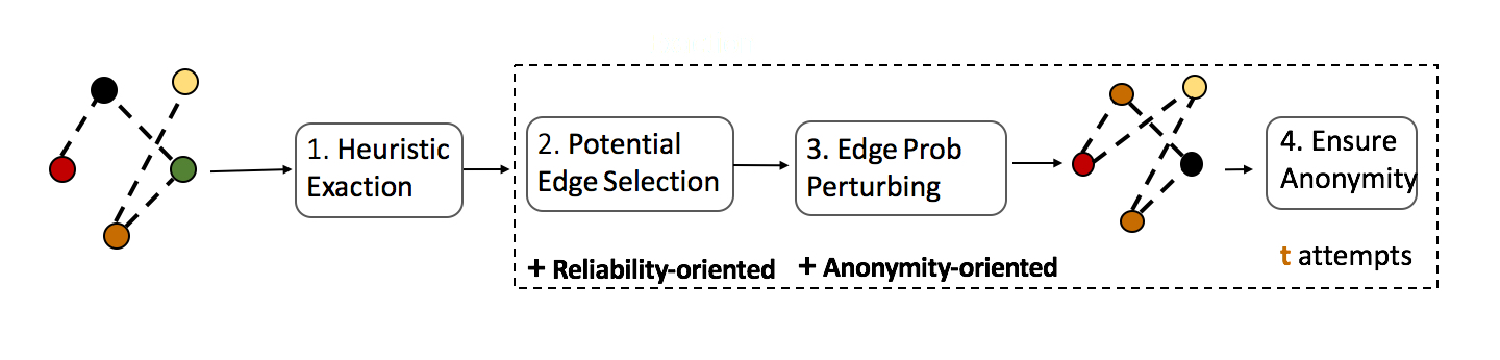
\includegraphics[scale=0.55]{figures/DegreeAUG/pipeline.eps}
    \caption{The pipeline of function \texttt{GenerateObfuscation}}
    \label{fig:genObfuscation}
\end{figure*}

Boldi {\etal}  proposed a seminal approach of anonymizing \emph{deterministic graphs} which injects uncertainty in the existence of the edges of the graph and publishes the resulting \emph{uncertain graph}. Their method injects uncertainty to edges in a deterministic graph as follows: for each existing sampled edge $e$, it is assigned a probability $1-r_{e}$, and for each non-existing sampled edge $e$, it is assigned a probability $r_{e} \leftarrow R_{\sigma_{e}}$.  By this way, it converts the input graph into an uncertain one. In particular, the perturbation variable $r_{e}$ is generated by a truncated $[0,1]$ normal distribution, $r_{e} \leftarrow R_{\sigma_{e}}$; 
\begin{equation*}
    R_{\sigma}(r):= \begin{cases}
                    \frac{\Phi_{0,\sigma}(r)}{\int_{0}^{1} \Phi_{0,\sigma}(x) dx} &  r \in [0,1] \\
                    0 &  \text{otherwise}
                    \end{cases}
     \label{eq:gen}
\end{equation*} 
where $\Phi_{0,\sigma}$ is the density function of a Gaussian distribution. 
As the standard deviation $\sigma$ of the normal distribution decreases, a greater mass of $R_{\sigma}$ will concentrate near $r=0$ and the amount of injected uncertainty will be smaller.  Namely, smaller values of $\sigma$ contribute towards better maintaining the characteristics of the original graph. Targeting at high utility, they formulated the graph anonymization problem as the minimization of $\sigma$ and computed the minimal amount of uncertainty via a binary search on the value of the uncertainty parameter $\sigma$. The overall anonymization procedure is illustrated in Algorithm \ref{alg:binarySearch}. 

The search flow of Algorithm \ref{alg:binarySearch} is determined by the function \texttt{GenerateObfuscation}, whose pipeline is shown as Figure \ref{fig:genObfuscation}. The function \texttt{GenerateObfuscation} aims to find a $(k,\epsilon)$-obfuscation of the original \emph{graph} using a given standard deviation parameter $\sigma$. A key feature of this function is the utilization of heuristics for judicious edge selection and edge prob perturbing. The function first computes heuristics values based on node properties in the input graph. After that, the search of $\keobf$ instance starts in a randomized way: $t$ attempts are performed. Each attempt performs the following steps:
\begin{itemize}
    \setlength\itemsep{0em}
	\item{Selecting a subset of edges $E_{c}$}
    \item{Perturbing existence probabilities of selected edges}
    \item{Checking the resulting uncertain graph whether satisfies the anonymity requirement}
\end{itemize}
If the algorithm finds a $(k,\epsilon)$-obfuscated graph in one of its $t$ trials, it returns the obfuscated graph with minimal $\epsilon$. Otherwise, the algorithm indicates the failure by returning $\tilde{\epsilon}=1$. 

\begin{sloppypar}
In this work, we extend this broad framework by incorporating its key function \texttt{GenerateObfuscation} with uncertainty. The specific method proposed in \cite{Boldi_Injecting_2012}, has two drawbacks for anonymizing uncertain graphs. First, their method does not consider the structural relevance of edges in the critical edge selection step, which leads to unnecessary structural distortion. Second, its interior edge perturbing mechanism assumes the existence of edges is known with certainty, thus fails to handle uncertain graphs where the existence of edges is probabilistic. We will present corresponding solutions (reliability-oriented edge selection and anonymity-oriented edge perturbing). 
\end{sloppypar}
\subsection{Reliability-oriented Edge Selection} 
\begin{sloppypar}
The most important step is the selection of potential edges, which impacts further anonymization effort significantly. Finding the optimal set of edges $E_{c}$ that balances privacy and utility is a typical combinational optimization problem. The problem is computationally expensive since there are exponential many combinations to be considered.     

To alleviate the combinational intractability, kind of heuristics have been utilized in the context of deterministic graphs. These heuristics can be classified into two main categories  (1) Anonymity-oriented ones that suggest implementing larger perturbation to less anonymized nodes~\cite{Ying2009} (2) Utility-oriented ones that suggest implementing smaller perturbation to more influential edges/nodes~\cite{casasprivacy,Ying_Randomizing_2008}. 
\end{sloppypar}

In this work, we present a sampling-based approach which combines both heuristics together. First, we adopt the idea of \emph{uniqueness score} for quantifying the anonymity level of nodes. Second, we introduce a novel edge relevance metric, \emph{reliability relevance} (RR), for quantifying the impact of edge modification to the overall uncertain graph. In contrast to the existing metrics such as edge betweenness~\cite{casasprivacy}, which are all defined in deterministic graphs, reliability relevance geared towards uncertain graphs. It allows us to select a subset of edges subjected to perturbation with less impact on reliability (reliability-oriented edge selection). 

\subsubsection{Uniqueness Score}
\label{sec:uniqueness}

\emph{Uniqueness score} is proposed to measure how typical the node is among all the nodes in terms of its property value \cite{Boldi_Injecting_2012}. More formally, the uniqueness score is defined as follows. 
\begin{definition}
    \textbf{Uniqueness Score~\cite{Boldi_Injecting_2012}}
     Let $P:V \rightarrow  \Omega_{P}$ be a property on the set of nodes $V$ of the graph $\mathcal{G}$, let $d$ be a distance function on $\Omega_{P}$, and let $\theta >0$  be a parameter. 
  Then the $\theta-commonness$ of the property values $\omega \in \Omega_{P}$ is $C_{\theta}(\omega):= \sum_{u \in V} \Phi_{0,\theta}(d(\omega, P(v)))$,   
while the $\theta$-uniqueness of $\omega \in \Omega_{P}$ is $U_{\theta}:= \frac{1}{C_{\theta}(\omega)}$. 
\end{definition} 
Note that, the commonness of the property value $\omega$ captures how typical the value $\omega$  is among all the  nodes in the graph via a weighted average function, where the weight decays exponentially as the distance $d$. As above defined, uniqueness scores depend on the parameter $\theta$, which determines the decay rate of average weights. In this work, we set $\theta=\sigma_{\mathcal{G}}$, where $\sigma_{\mathcal{G}}$ represents how frequently the property value spread in the uncertain graph $\mathcal{G}$. A comprehensive discussion can be found in the literature \cite{Boldi_Injecting_2012}.

\subsubsection{Reliability Relevance}

\begin{figure}[!tb]
    \begin{subfigure}[b]{0.45\textwidth}
        \centering
         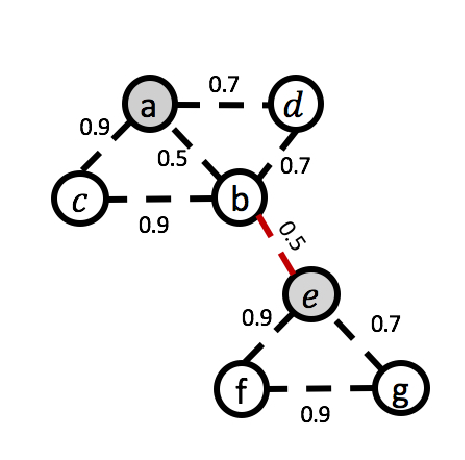
\includegraphics[scale=0.4]{figures/DegreeAUG/uncertainO.eps}
         \caption{\small{An uncertain graph}}
        \label{fig:edgeBridgeGraph}
    \end{subfigure}
    \begin{subfigure}[b]{0.45\textwidth}
        \centering
         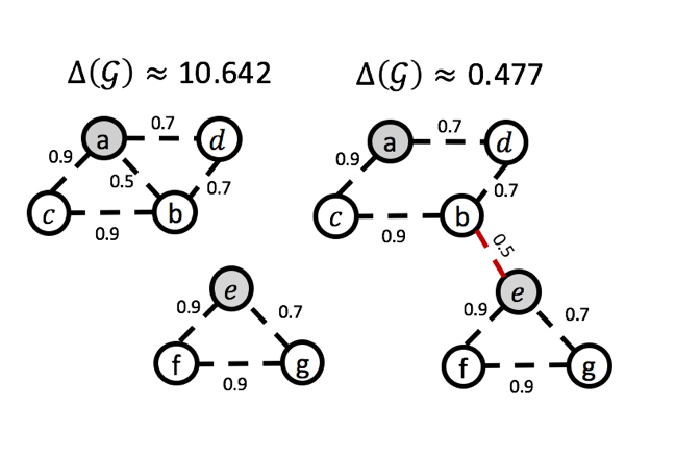
\includegraphics[scale=0.4]{figures/DegreeAUG/uncertainC.eps}
         \caption{\small{Resulting uncertain graphs}}
        \label{fig:edgeRelevance}
     \end{subfigure}
     \caption{Illustration of varying structural distortions by removing different uncertain edges $(b,e)$ and $(a,b)$ over an uncertain graph.}
     \label{fig:edgeRR}
\end{figure}
As exemplified in Figure~\ref{fig:edgeRR}, each edge modification will have \emph{varying} impact to the graph structure in the context of uncertain graphs. From the perspective of \emph{uniqueness}, nodes $a$ and $e$ are identical since adjacent edges have identical uncertainties. Accordingly, anonymity-oriented heuristics would select and perturb edges $(a,b)$ and $(b,e)$ without bias. As shown in Figure~\ref{fig:edgeRR}, the deletion of the uncertain edge $(b,e)$, the only link connecting two \emph{reliable} clusters, clearly incurs much larger structure distortion than the deletion of the edge $(a,b)$. This observation calls for an effective measure of edge influence in the context of uncertain graphs. 

Inspired by the significance of \emph{reliability}, we provide a compact analytic form of reliability deviation caused by individual uncertain edge modification in a fine-grained way, namely changing its edge probability in any granularity. Following the path, we introduce edge reliability relevance for edges' influence estimation, which can be quantified by the sum of reliability discrepancy of all the node pairs. Besides, we provide an algorithm for accessing edge \emph{reliability relevance} (RR) efficiently. 

\paragraph{Reliability Relevance Definition}

Lets start with analyzing the impact of single uncertain edge alteration to the connectivity of a specific node pair (Two-terminal Reliability).  
\begin{definition}
    \textbf{Two-terminal Reliability Relevance}
    Given an uncertain graph $\mathcal{G}$, and two nodes $u,v$, we consider the probability that $u$ is reachable to $v$,$R_{u,v}(\mathcal{G})$, as defined in Definition \ref{d:reliability}, as a multivariate function involving all the edge probabilities.   
    Thus, the partial derivative of $R_{u,v}(\mathcal{G})$ with respect to an individual variable $p(e)$, existence probability of an uncertain edge, denotes as $RR_{u,v}(e)$. It represents the sensitivity to the change of reliability $R_{u,v}$ which is determined by $p(e)$ with the others held constant. Its definitions is as follows:  
\begin{equation*}
    \svj
    RR_{u,v}(e)= \frac{\partial R_{u,v}(\mathcal{G})}{\partial \mathit{p}(e)}
    \svj
\end{equation*}
\end{definition}

% The following factorization lemma underlies the computation of partial derivative $RR_{u,v}(e)$ in a compact form. 
\begin{lemma}
    \textbf{Factorization Lemma}
       Given an uncertain graph $\mathcal{G}$, the reliability of the node pair $(u,v)$ $R_{u,v}(\mathcal{G})$ can factorized via one uncertain edge $e$ as follows:
    \vj
    \begin{equation*}
        R_{u,v}(\mathcal{G}) = p(e) R_{u,v} (\mathcal{G}_{e}) + (1-p(e)) R_{u,v} (\mathcal{G}_{\bar{e}} )
        \label{eq:fac}
        \svj
    \end{equation*}
    where uncertain graph $\mathcal{G}_{e}$ is identical with $\mathcal{G}$ except its edge $e$ is an \textbf{certain} edge. Similarly, the uncertain graph $\mathcal{G}_{\bar{e}}$ is identical with $\mathcal{G}$ except its edge $e$ is an \textbf{certain non} edge. 
\end{lemma}
According to the factorization lemma, the partial derivative $RR_{u,v}(e)$ can be rewritten as 
\vj
\begin{equation*}
    RR_{u,v}(e)=R_{u,v}(\mathcal{G}_{e})-R_{u,v}(\mathcal{G}_{\bar{e}})
\end{equation*}
\svj
The equation indicates the sensitivity of reliability is constant and it does not depend on the probability value of the uncertain edge $e$. Another important point to remember is that because all the connected pairs remain connected after the addition of an edge, $R_{u,v}(\mathcal{G}_{e}) - R_{u,v} (\mathcal{G}_{\bar{e}}) \ge 0$.

For a given uncertain edge $e$, the derivatives $RR_{u,v}(e)$ can be arranged in a $|V|\times |V|$ matrix, where each element corresponds to one node pair $(u,v)$ and it gives the partial derivative for the corresponding reliability $R_{u,v}$. As ever discussed, all the element are equal to or greater than zero.  
In this work, we define $RR(e)$ to be reliability relevance of an edge $e$ which can be quantified by the sum of all the $RR_{u,v}(e)$, as  
\vj
\begin{align*}
    RR(e) &= \sum_{u,v} |RR_{u,v}(e)| \\
          &= \sum_{u,v} |R_{u,v}(\mathcal{G}_{e}) -R_{u,v}(\mathcal{G}_{\bar{e}})| \\  
         &= \sum_{u,v} R_{u,v} (\mathcal{G}_{e}) - \sum_{u,v} R_{u,v}(\mathcal{G}_{\bar{e}})
    \svj 
\end{align*}
Note that, $RR(e)$ equals the difference of the expected number of connected pairs between uncertain graphs $\mathcal{G}_{e}$ and $\mathcal{G}_{\bar{e}}$ by explicit incorporation of edge uncertainty. In the context of edge relevance, reliability relevance can be seen as generalization of cut-edges, which quantifies the impact of partial edge deletion or addition on the connectivity in the uncertain graph. 
The higher reliability relevance score of an edge, the bigger impact of edge perturbation over the overall graph.  
On this basis, we define the reliability centrality of node $v$,$RC(v)$ to be the overall influence of graph reliability which can be quantified by the weighted sum of reliability relevance of all adjacent edges. 
\svj
\begin{equation*}
    RC(u)=\sum_{e} p(e) RR(e)
    \svj
\end{equation*}

\begin{algorithm}[!tb]
    \begin{algorithmic}[1]
       \item[] {\textbf{Input:} ~$\mathcal{G}=(V,E,\mathit{p})$, $K$ is the number of sampled graphs; usually $K=1000$}
    \item[] {\textbf{Output:} ~$RR$ Reliability relevance of edges in $\mathcal{G}$}
    \STATE {$CC_{e} \leftarrow  \mathbf{0} $, $CC_{\bar{e}} \leftarrow \mathbf{0}$}
    \FOR{i=1 \TO K }
    \STATE {$G \leftarrow $  A deterministic sampled instance}
    \STATE {$Ind(G)$ is edge existence of sampled graph $\mathcal{G}$}
    \STATE {$cc(G) \leftarrow $ the number of connected pairs of $G$}
    \STATE {$CC_{e}+=Ind(G) \cdot cc(G)$,$CC_{\bar{e}}+=(\mathbf{1}-Ind(G)) \cdot cc(G)$ }
    \ENDFOR
    \STATE{$RR= CC_{e}/\mathit{p} - CC_{\bar{e}}/{\mathbf{1}-\mathit{p}}$}
         \caption{Reliability Relevance Evaluation}
        \label{alg:RReval}
    \end{algorithmic}
\end{algorithm}


\paragraph{Reliability Relevance Evaluation}

Note that, the evaluation of $RR(e)$ need computing all the $R_{u,v}$ over two uncertain graphs $\mathcal{G}_{e}$ and $\mathcal{G}_{\bar{e}}$.  The two-terminal reliability detection problem is a $\#$P-complete problem \cite{MOBall}. Thus, the exact computation is not practical for large uncertain graphs. A basic approach is to get reliability approximation by sampling: for each uncertain edge $e$ 1) we first sample $K$ possible graphs $G_{1}, \ldots G_{K}$ of $\mathcal{G}_{\bar{e}}$ according to edge probability $\mathit{p}$, and 2) we then compute the number difference of connected pairs in each sample graph after edge $e$ is added. The basic sampling method can be rather computationally expensive. The total running time is $\Theta(|E| \cdot K\cdot \alpha(|V|) |E|)$ assuming incremental algorithm is used for computing connected components. It is impractical for large uncertain graphs with huge size of edges. 

Here, we introduce a much faster approach for computing $RR(e)$ as shown in Algorithm \ref{alg:RReval}. The basic idea is to partition all sampled graphs into groups according to existing edges so that the evaluation of the number of connected pairs can be reused. 
The complexity of reliability relevance evaluation of all edges is  $\Theta(K \cdot \alpha(|V|) |E|)$. 

\subsubsection{Reliability-oriented Edge Selection Procedure}

\begin{algorithm}[t!]
	\begin{algorithmic}[1]
    	\item[] {\textbf{Input:}~Uncertain graph $\mathcal{G}=(V,E,\mathit{p})$, $ak,k,\epsilon,c,q$, \\and standard deviation $\sigma$ }
        \item[] {\textbf{Output:}~A pair $\langle \tilde{\epsilon}, \tilde{\mathcal{G}} \rangle$} 
        \STATE  {\textbf{compute} the uniqueness $U(v)$ for all the nodes}
        \STATE  {\textbf{compute} the \texttt{centrality} $RC(v)$ for all the nodes}
        \STATE  {$Q(v) \leftarrow U(v) \cdot RC(v)$}
        \STATE {$H \leftarrow$  the set of $\lceil \frac{\epsilon}{2} |V| \rceil$ with largest $Q(v)$}
        \COMMENT{Excluding}
     	\STATE {Normalized $RC(v)$; $Q(v) \leftarrow U(v) \cdot 1-RC(v)$;}
        \STATE {$\tilde{\epsilon} \leftarrow 1$}
   		\FOR{$t$ times} 
        	\STATE {$E_{C} \leftarrow E$} % either it become probabilistic 
            \COMMENT{Reliability-oriented Edge Selection}
         	\REPEAT  
            	\STATE{randomly pick a vertex $u \in V \setminus H$ according to $Q$}
            	\STATE{randomly pick a vertex $v \in V \setminus H$ according to $Q$}
            	\STATE{draw $w$ uniformly at random from $[0,1]$} 
            \IF {$(u,v) \in E$} 
				\IF {\texttt{$w > p(e)$}} 
                	\STATE {$E_{C} \leftarrow E_{c} \setminus \lbrace(u,v)\rbrace$}
                \ENDIF
            \ELSE \STATE{$E_{c} \leftarrow E_{c} \cup \lbrace(u,v)\rbrace$}
            \ENDIF 
            \UNTIL{$E_{C}=c|E|$}
            \FORALL {$e \in E_{C}$} 
            	\STATE {\textbf{compute} $\sigma(e)$}
                \COMMENT{Edge Probability Perturbation}
                \STATE {draw $w$ uniformly at random from $[0,1]$}
				\IF {$w < q$} \STATE{$r_{e} \leftarrow U(0,1)$}
                \ELSE 
                \STATE{$r_{e} \leftarrow R_{\sigma(e)}$}
                \ENDIF
                \STATE \textbf{$\tilde{p}(e) \leftarrow p(e)+ 2(0.5-p(e))\cdot r_{e}$}
            \ENDFOR
            \STATE {$\hat{\epsilon} \leftarrow checkAnonymity(\tilde{\mathcal{G}})$} 
            \COMMENT{Ensure Anonymity}
           	\STATE {Update result $\langle \tilde{\epsilon}, \tilde{\mathcal{G}} \rangle$ if $\hat{\epsilon}<\tilde{\epsilon}$}
        \ENDFOR 
        \STATE {return $\langle \tilde{\epsilon}, \tilde{\mathcal{G}} \rangle$}
      	\caption{GenerateObfuscation}
        \label{alg:genObf}
    \end{algorithmic}
\end{algorithm}
Now, we are ready to introduce our function \texttt{GenerateObfuscation} aims at finding a $(k,\epsilon)$-obf instance for an input \emph{uncertain graph} $\mathcal{G}$ using a given standard deviation parameter $\sigma$ as shown in Algorithm \ref{alg:genObf}. It resembles the method proposed in \cite{Boldi_Injecting_2012} with explicit incorporation of edge uncertainty in edge selecting and perturbing step. Another important contribution of our work is the utilization of reliability relevance (RR) for capturing structural relevance of edges in the uncertain graph.  

First, it computes the uniqueness level and reliability centrality for each node $v \in \mathcal{G}$. Intuitively, the more unique a node is, the harder it is to be obfuscated; the more \emph{important} an edge is, the bigger utility loss it incurs. Such heuristic information is important for our privacy-preserving and utility-preserving purpose. In order to  use the ``uncertainty budget'' in the most efficient way, the algorithm performs the following steps as shown in Algorithm \ref{alg:genObf}.

(Line 4: Excluding) Since it is allowed not to obfuscate $\epsilon|V|$ of the nodes, the algorithm selects the set $H$ of $\frac{\epsilon}{2}|V|$ nodes with largest uniqueness scores or reliability centrality scores, and exclude them from the subsequent obfuscation efforts. In later steps, the algorithm will inject uncertainty only to edges that are not adjacent to any of vertices in $H$. The key feature of our method is that it strictly preserve the 1-neighborhoods of influential nodes.  

(Line 8-18: Potential Edge Selection) The set of nodes not in $H$ will need to be anonymized. To anonymize more unique vertices, higher uncertainty is necessary. Thus, edges needed to be sampled with higher probability if they are adjacent to unique nodes. In order to better preserve graph structure, edges needed to be sampled with smaller probability if they are adjacent to more influential nodes. In order to handle this sample process, our algorithm assigns a probability $Q(v)$ to every $v \in V$, which depends on the uniqueness level $U(v)$ and reliability centrality $RC(v)$ of $v$. 

Each attempt begins by selecting a subset of edges $E_c$, which will be subjected to edge probability perturbation. Then set $E_{c}$, whose target size $\norm{E_c}=c \norm{E}$, is initialized to be $E$. Then, the algorithm randomly selects two distinct vertices $u$ and $v$, according to probability distribution $Q$. The pair of vertices $(u,v)$ is removed from $E_{c}$ with the probability $p(e)$ if it is an edge in the original graph, or added to $E_{c}$ otherwise.  The process is repeated until $E_{c}$ reaches the require size. In typical uncertain graphs, the number of non-edges is significantly larger than the number of uncertain edges, the loop ends very quickly, for small values of $c$. And, the resulting set $E_{c}$ includes most of edges in $E$. 

(Line 20) Next, we redistribute the perturbation budget among all selected edges $e \in E_{c}$ in proportion to their intermediate representations $Q(v)$. Specially, we define for each $e=(u,v) \in E_{c}$ , its uncertainty level, 
\vj
\begin{equation*}
Q(e):= \frac{Q(u)+Q(v)}{2}
\svj
\end{equation*}
and then set its edge perturbation parameter 
\vj
\begin{equation*}
\svj
\sigma(e)=\sigma |E_{c}|  \cdot \frac{Q(e)}{\sum_{e \in E_{c}} Q(e)}
\end{equation*}
so that the average of $\sigma(e)$ over all $e \in E_{C}$ equals $\sigma$.
\subsection{Anonymity-oriented Edge Perturbing}
\begin{figure}
    \captionsetup{justification=centering,margin=1cm}
       \begin{subfigure}[b]{0.45\textwidth}
        \centering
        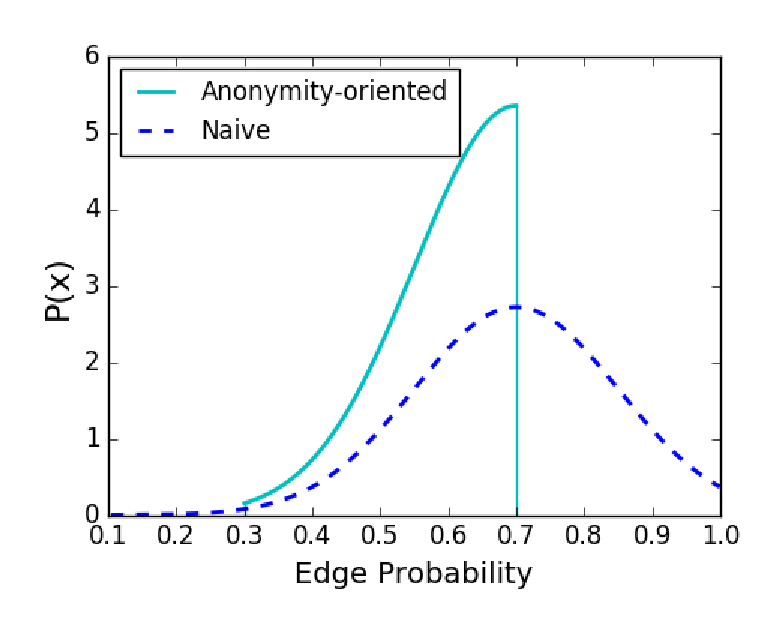
\includegraphics[scale=0.35]{figures/DegreeAUG/AnonymityEP.eps}
        \caption{\small{Anonymity-oriented Edge Perturbing}}
        \label{fig:anonymityEP}
    \end{subfigure}%
    \centering
        \begin{subfigure}[b]{0.45\textwidth}
            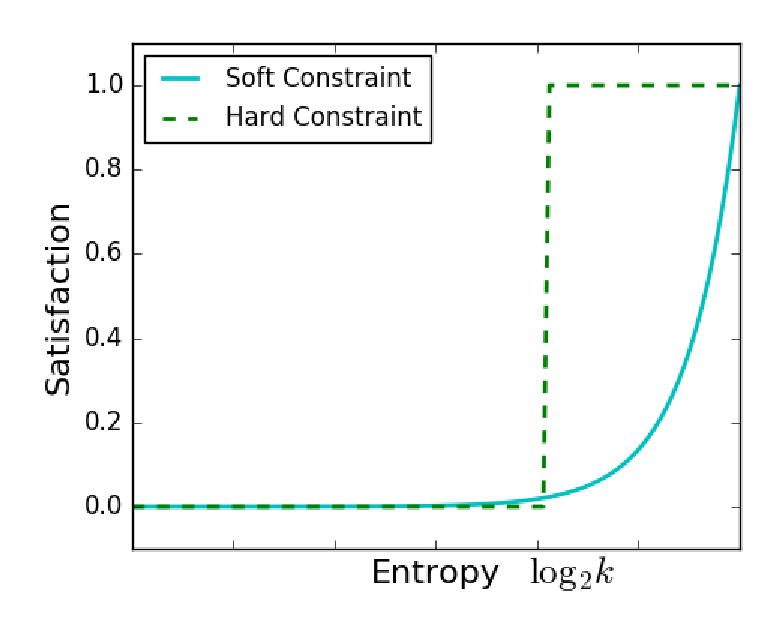
\includegraphics[scale=0.35]{figures/DegreeAUG/constraint.eps}
            \caption{\small{Relaxing $k$-obfuscation constraint}}
            \label{fig:constraintRelax}
        \end{subfigure} 
\end{figure}
As ever discussed, the existing uncertainty injecting scheme is designed for deterministic graphs and can not be used to handle uncertain graphs directly. Given the uncertainty level $\sigma(e)$, a natural strategy is to consider the partial edge addition and deletion in a random way as shown in Figure \ref{fig:anonymityEP}. Through the analysis of the impact of a single edge probability alteration, we give a anonymity-oriented perturbing heuristics which is able to constraint the potential range of edge prob perturbing (referred to C). For each selected edge $e \in E_{c}$ and the assigned uncertainty level $\sigma(e)$, we alter its existence probability as 
\vj
\begin{equation*}
    \tilde{\mathit{p}}(e):=\mathit{p}(e) + (1-2 \mathit{p}(e)) \cdot r_{e} 
    \svj
\end{equation*} 
Where the random perturbation $r_{e}$ is generated according to $\sigma(e)$ as Eq. \ref{eq:gen}. Namely, for an edge with the probability $p$, we only consider potential edge probability $\tilde{p}$ in the limited range that more likely contributes to higher graph anonymity. Clearly, previous scheme defined in deterministic graph becomes a special case of our approach. We proceed to elaborate the rationality and the benefit of this anonymity-oriented edge perturbing scheme by treating it as a constraint satisfaction problem. 
  
\subsubsection{Basics}
Let us consider $k$-obfuscate a given node $v$ as a single constraint $c_{v}$ for the target anonymization graph. Then, according to the definition \ref{obfCon}, the satisfaction of the constraint $c_{v}$ is defined as
\begin{equation*}
    \mathtt{c}_{v}:=
        \begin{cases}
                1  & H(Y_{P(v)}) \geq \log_{2}{k} \\
                0  & otherwise \\
         \end{cases}
\end{equation*}
Namely, given the considered degree-based re-identification scenario, we lower bound the entropy of degree distribution over the anonymized graph by $log_{2}{k}$. Accordingly, whether the anonymized graph $k$-obfuscates all the nodes can be expressed as degree of joint satisfaction.
\vj
\begin{align*}
    \mathcal{C(\mathcal{G})} &= \prod_{v \in V} \mathtt{c}_{v} \\
                &=\prod_{\omega} \underbrace{\mathtt{c} \ldots \mathtt{c}}_{s(\omega)}
    \svj
\end{align*}
The uncertain graph is said to $k$-obfuscate all the nodes if and only if the $C(\mathcal{G})$ equals 1.  
\subsubsection{Re-visiting graph anonymity}
As shown in Figure \ref{fig:constraintRelax}, the original satisfaction function is not everywhere differentiable.To simply the anonymity analysis, we approximate the individual constraint $c_{v}$ to a fuzzy relation in which the satisfaction degree of a constraint is defined as a continuous and differentiable function, going from fully violated to fully satisfied. A natural candidate for soft satisfaction function is,
\svj  
\begin{equation*}
    C_{v} = e^{H(Y_{P(v)})-\log_{2}{|V|}}
    \svj
\end{equation*}
According to this approximation, the satisfaction function of $k$-obfuscate all the nodes can be rewritten as
\svj
\begin{equation*}
   \mathcal{C}(\mathcal{G}) \propto \prod_{\omega} \underbrace{e^{H(Y(\omega)} \ldots e^{H(Y(\omega))}}_{s(\omega)}
\end{equation*}
While the original satisfaction is a binary value, the approximated satisfaction value lies in the continuous range $[0,1]$. Note that, the higher satisfaction score indicates the higher level of anonymity achieved. Taking logarithm for both side, we get the concise formula as 
\svj
\begin{equation*}
    \log \mathcal{C}(\mathcal{G})=\sum_{\omega} s(\omega) \cdot H(Y(\omega)
\end{equation*}
Regarding the property $P$, it equals the weighted sum of entropy over all possible values $\omega$, where $s(\omega)$ is the expected number of vertices with property value $\omega$ over all possible worlds. Targeting at high anonymity, we wish to increase the weighted sum of entropy. 

\subsubsection{Greedy search of graph anonymity}
% \begin{figure}
%     \centering
%     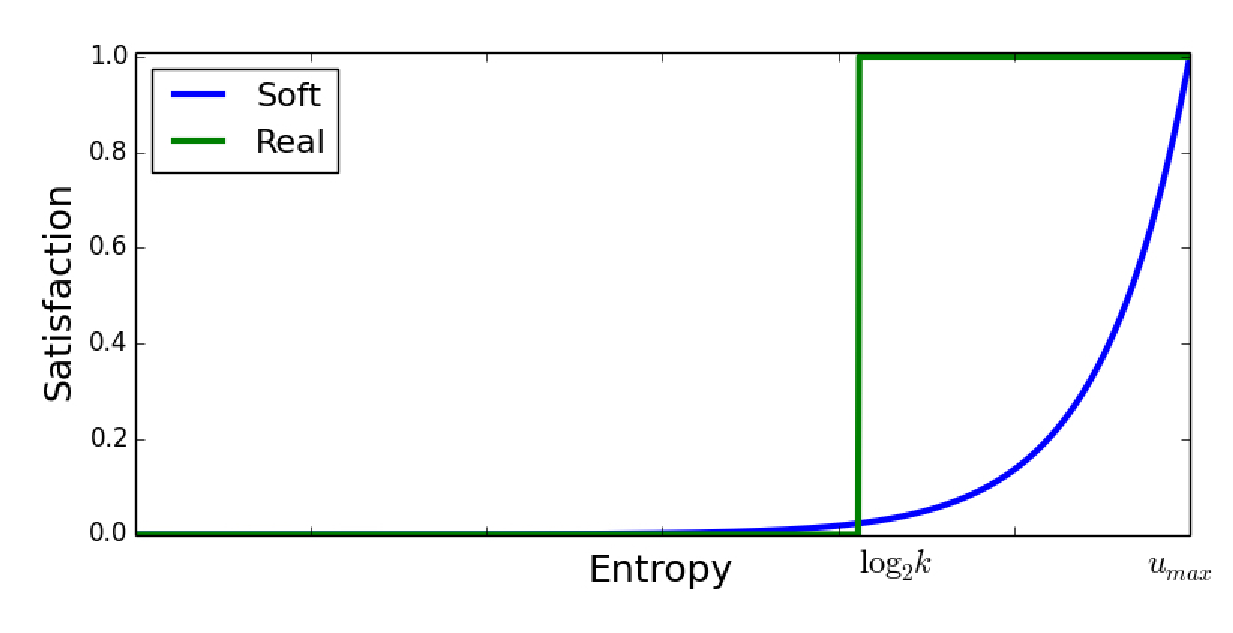
\includegraphics[scale=0.3]{figures/fuzzyConstraint.eps}
%     \caption{Relaxing Constraint}
%     \label{fig:rc}
% \end{figure}
The remaining issue is to connect the single edge probability alteration with the objective. With respects to node degree, a graph can be represented as one matrix as shown in figure \ref{fig:constraintRelax}. The weighted sum of entropy is related with graph coding. Here, we utilize entropy encoding, especially Huffman coding. From the coding perspective, we have two different angles to perform graph coding: row or column of degree matrix. The encoded length should be equal to each other, as shown in the following equation.  
\svj
\begin{equation*}
    \sum_{v} H(v) + n \log{n} = \sum_{\omega} s(\omega) \cdot H(Y(\omega))+ H(s(\omega))
    \svj
    \label{wegithedEn}
\end{equation*}
It indicates that higher global anonymity of a uncertain graph can be achieved by increasing the entropy of individual nodes when the global distribution $H(\omega)$ keeps constant. 

Note that, the probability change over a specific edge only affects degree distributions of its connected nodes. 
To further simply the problem, we assume that the impact of edge perturbing is independent to each other. Recall that, we suggest implementing perturbation to less anonymized nodes. In the case of degree obfuscation, they are nodes with high degree. For a node $v$ with high degree, the probability distribution of its degree $d_{v}$ may be approximated as the normal distribution as implied by the Central Limit Theorem. Hence, its induced entropy $H(v)$ can be approximated as $\frac{1}{2} {\ln (2 \pi e \sigma^2)}$. 

Targeting at maximizing the graph anonymity, we take steps proportion to the positive gradient with respect to the choice of individual edge probabilities. 
\svj
\begin{equation*}
    \frac{\partial \sum_{\omega} s(\omega) H(Y(\omega))} {\partial p(e)} \propto (1-2\mathit{p}(e))  
\end{equation*} 
Therefore, 
\vj
\begin{equation*}
    \tilde{\mathit{p}}(e):=\mathit{p}(e) + (1-2 \mathit{p}(e)) \cdot r_{e}
\end{equation*} 
Namely, our approach simulates one iteration of batch gradient ascent method for finding the local maximum of weighted entropy sum or the anonymity level. 
% \begin{algorithm}[t!]
	\begin{algorithmic}[1]
    	\item[] {\textbf{Input:}~Uncertain graph $\mathcal{G}=(V,E,\mathit{p})$, $ak,k,\epsilon,c,q$, \\and standard deviation $\sigma$ }
        \item[] {\textbf{Output:}~A pair $\langle \tilde{\epsilon}, \tilde{\mathcal{G}} \rangle$} 
        \STATE  {\textbf{compute} the uniqueness $U(v)$ for all the nodes}
        \STATE  {\textbf{compute} the \texttt{centrality} $RC(v)$ for all the nodes}
        \STATE  {$Q(v) \leftarrow U(v) \cdot RC(v)$}
        \STATE {$H \leftarrow$  the set of $\lceil \frac{\epsilon}{2} |V| \rceil$ with largest $Q(v)$}
        \COMMENT{Excluding}
     	\STATE {Normalized $RC(v)$; $Q(v) \leftarrow U(v) \cdot 1-RC(v)$;}
        \STATE {$\tilde{\epsilon} \leftarrow 1$}
   		\FOR{$t$ times} 
        	\STATE {$E_{C} \leftarrow E$} % either it become probabilistic 
            \COMMENT{Reliability-oriented Edge Selection}
         	\REPEAT  
            	\STATE{randomly pick a vertex $u \in V \setminus H$ according to $Q$}
            	\STATE{randomly pick a vertex $v \in V \setminus H$ according to $Q$}
            	\STATE{draw $w$ uniformly at random from $[0,1]$} 
            \IF {$(u,v) \in E$} 
				\IF {\texttt{$w > p(e)$}} 
                	\STATE {$E_{C} \leftarrow E_{c} \setminus \lbrace(u,v)\rbrace$}
                \ENDIF
            \ELSE \STATE{$E_{c} \leftarrow E_{c} \cup \lbrace(u,v)\rbrace$}
            \ENDIF 
            \UNTIL{$E_{C}=c|E|$}
            \FORALL {$e \in E_{C}$} 
            	\STATE {\textbf{compute} $\sigma(e)$}
                \COMMENT{Edge Probability Perturbation}
                \STATE {draw $w$ uniformly at random from $[0,1]$}
				\IF {$w < q$} \STATE{$r_{e} \leftarrow U(0,1)$}
                \ELSE 
                \STATE{$r_{e} \leftarrow R_{\sigma(e)}$}
                \ENDIF
                \STATE \textbf{$\tilde{p}(e) \leftarrow p(e)+ 2(0.5-p(e))\cdot r_{e}$}
            \ENDFOR
            \STATE {$\hat{\epsilon} \leftarrow checkAnonymity(\tilde{\mathcal{G}})$} 
            \COMMENT{Ensure Anonymity}
           	\STATE {Update result $\langle \tilde{\epsilon}, \tilde{\mathcal{G}} \rangle$ if $\hat{\epsilon}<\tilde{\epsilon}$}
        \ENDFOR 
        \STATE {return $\langle \tilde{\epsilon}, \tilde{\mathcal{G}} \rangle$}
      	\caption{GenerateObfuscation}
        \label{alg:genObf}
    \end{algorithmic}
\end{algorithm}


\section{Contribution List}
To the best of our knowledge, we are the first to deal with uncertain graph anonymization aiming at less reliablity change. Our contrinutions inlcudes:
\begin{itemize}
\itemsep0em 
\item{We identify and formalize the new and important problem of privacy preserving publication of uncertain graphs.
	We design a new framework, namely {\em AUG}, for efficient anonymization of uncertain graphs under the {\keobf} anonymization principle. 
	{\em AUG} integrates the edge uncertainties throughout the anonymization process to ensure the desired privacy level.}

\item{We show case that a naive approach that combines existing techniques from literature for uncertain graph 		anonymization do not work in practice due to significant utility loss. 
}

\item{We introduce a new reliability-based utility metric for assessing the utility loss during the anonymization process. We propose uncertainty-aware heuristics for injecting noise and perturbing the graph structure to anonymize the uncertain graph while minimizing utility loss.}	
	
\item{
We perform an extensive experimental evaluation using four real-world uncertain graph data sets from different  domains. We evaluate {\em AUG} using different groups of graph metrics. The results demonstrate a significant advantage of the proposed framework over the naive conventional methods, which do not directly consider edge uncertainty. 
}
\end{itemize}